\chapter{Results}
\label{chap:results}
In this chapter the results of the classification using “Max MCC” optimization strategy are presented. Some premises are necessary before proceeding with the interpretation of the data:

\begin{figure}[h!]
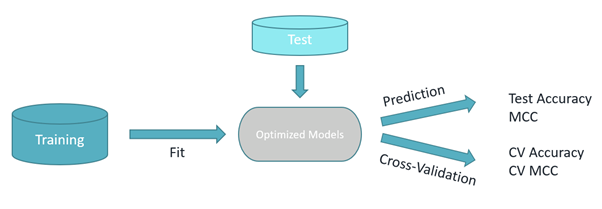
\includegraphics[width=12cm]{img/methods/data_split_strategy.png}
\centering
\caption{Approach used to compute Test Accuracy, MCC, CV Accuracy and CV MCC with separate splits of data.} \label{fig_data_split_strategy}
\end{figure}

\begin{enumerate}
\item 	The average scores at the bottom of each table are between models with the same architecture, but different hyper-parameters. Furthermore, having an accuracy lower than the chance level but with a positive \ac{MCC} has been preferred compared to have the highest possible accuracy with a zero or negative \ac{MCC}.
\item 	CV Accuracy, CV Acc Std, \ac{CV MCC} and CV MCC Std stand for Cross-Validated Accuracy and MCC and their respective standard deviation.
\item 	Test accuracy and \ac{MCC} are computed using an unseen test split of the data. CV Accuracy and \ac{CV MCC} have been computed on the training split of the data; thus, their purpose is to provide a measure of consistency of the test scores (see Fig \ref{fig_data_split_strategy}).
\item 	The confidence interval has been calculated on the test split, Z=1.96. Chance level represents the default guessing of the majority class.
\end{enumerate}

First, the classification performances of \ac{SVM} and \ac{MLP} are compared for both arousal and valence classification. Then, the performances between “Max MCC” and “Max Accuracy” strategies are compared, and the criteria to choose “Max MCC” as preferred one are explained. Finally, the results are compared with related work.

\section{Support Vector Machines vs Multi-Layer Perceptron}
\label{sec:svm_mlp}
The results of the subject-dependent arousal classification experiment are reported in Table \ref{tbl:arousal_results}, while the results for valence classification are reported in Table 2. In arousal classification, the highest and consistent test accuracy score is 81\% with \ac{MCC} score of 0.61 using \ac{SVM} and 80\% with \ac{MCC} score of 0.61 using \ac{MLP}. The 5 highest consistent accuracy scores for each classifier have been highlighted in light blue for comparison. \ac{SVM} obtained higher average test accuracy score of 63\% (0.09) and average \ac{MCC} score of 0.18 (0.20), with only 5 models scoring \ac{MCC} \(\leq 0 \) and no model scoring \ac{CV MCC} \(\leq 0\), while for \ac{MLP}  7 models scored \ac{MCC} \(\leq 0\) and 6 models scored scoring \ac{CV MCC} \(\leq 0\).

\begin{table}[h!]
  \caption{Arousal classification results using MCC as scoring parameter for GridSearch. The 5 best performing models in terms of accuracy and MCC score are highlighted in blue, the models with MCC \(\leq 0 \) or CV MCC \(\leq 0\) are highlighted in orange and yellow, respectively.}
  \label{tbl:arousal_results}
  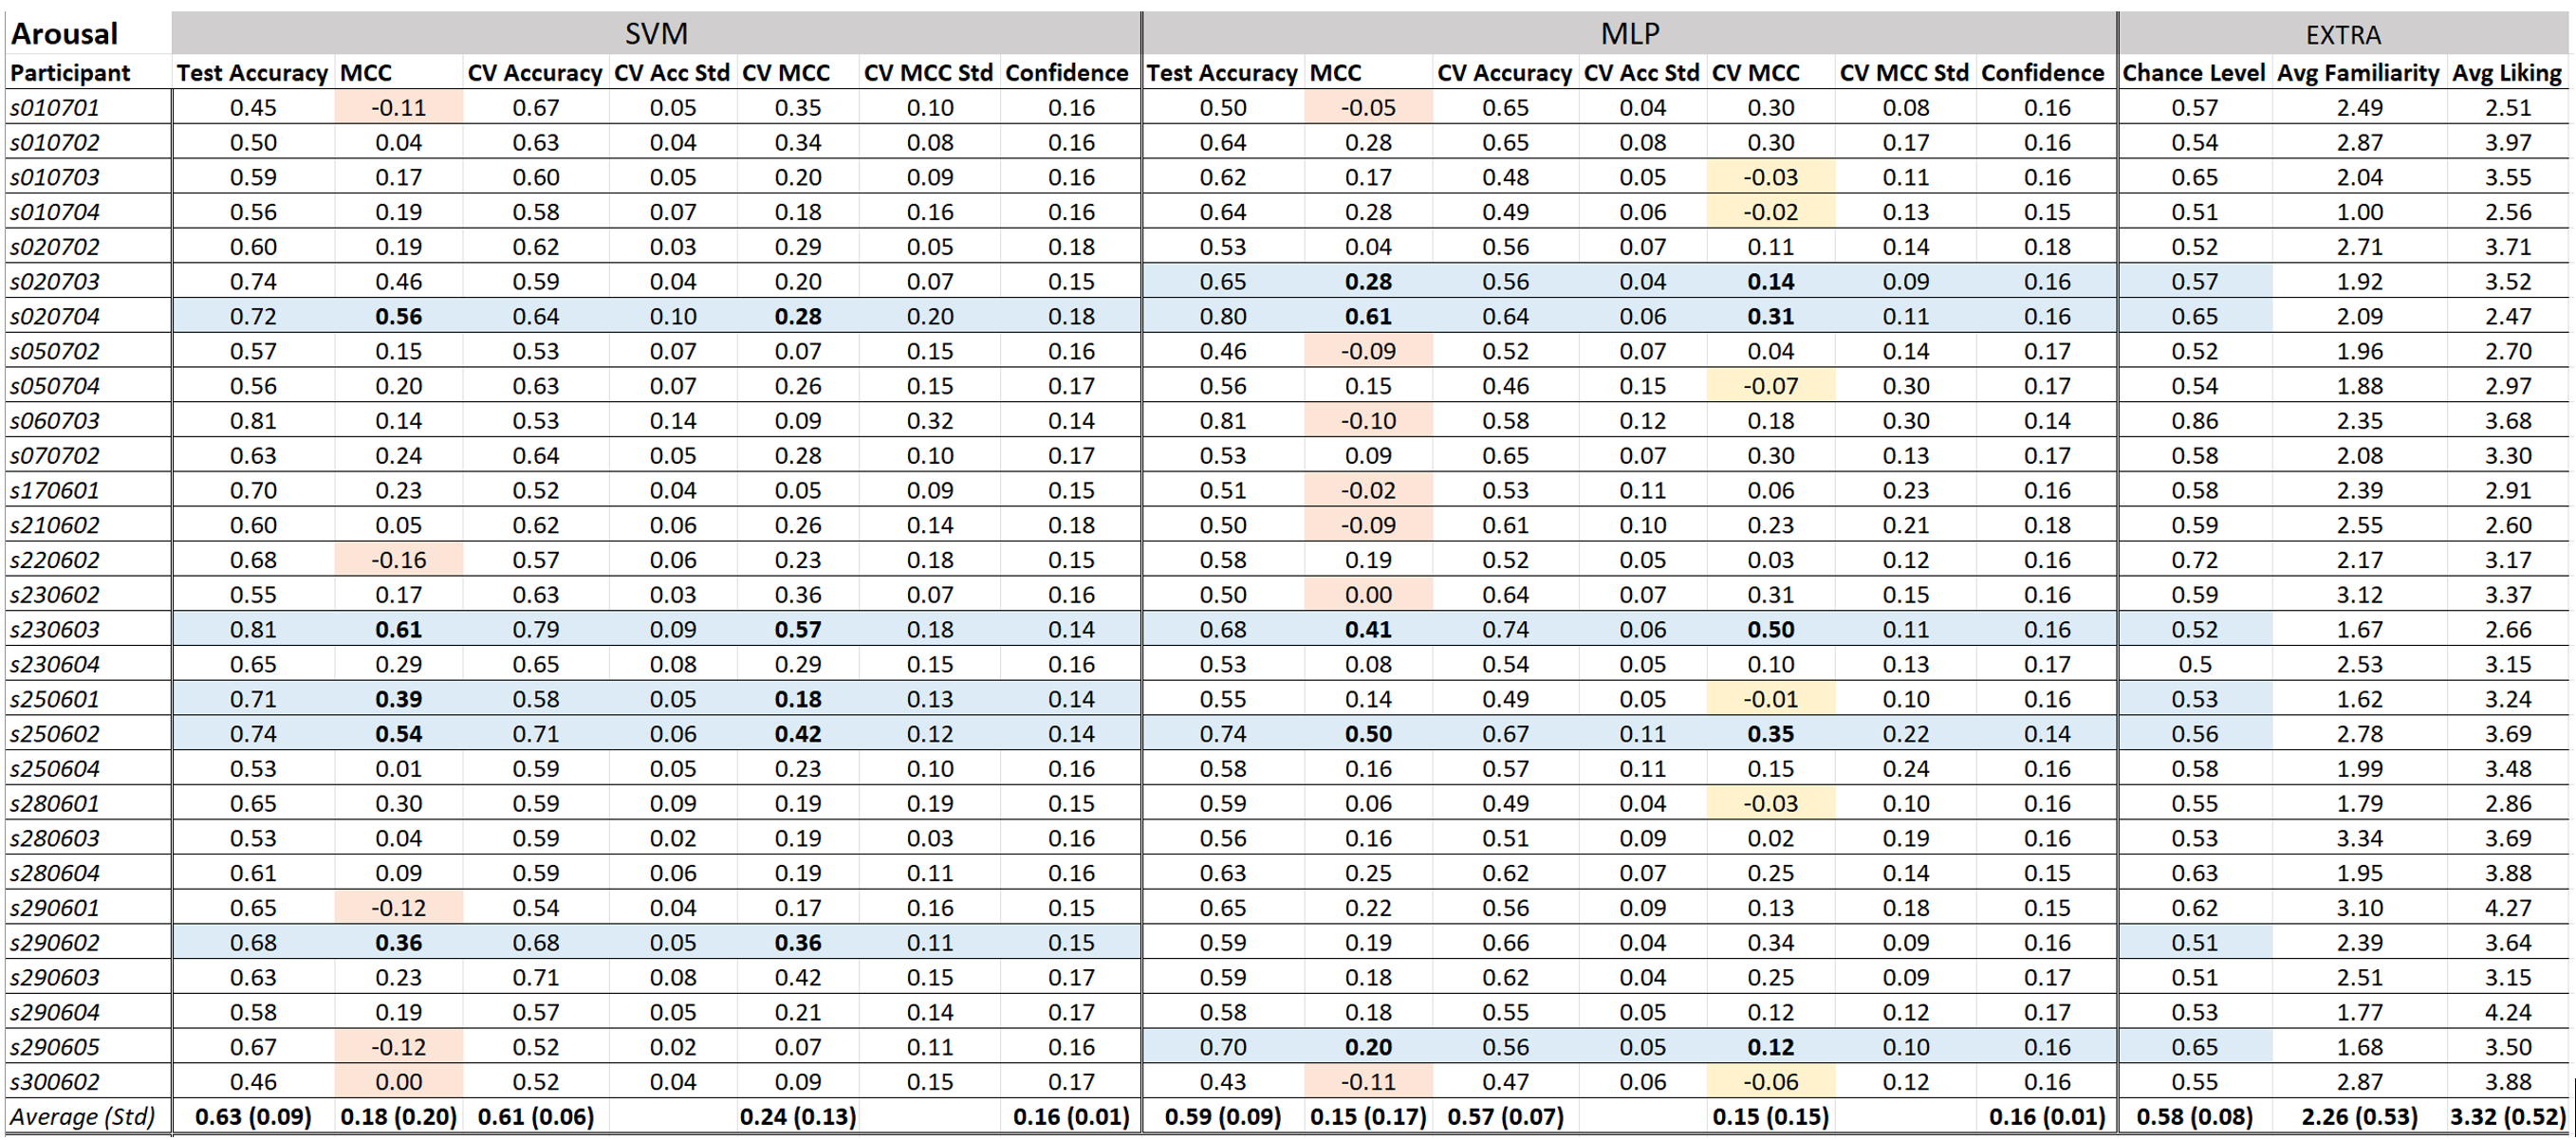
\includegraphics[width=\linewidth]{img/results/arousal_results.png}
\end{table}

For valence classification (see Table \ref{tbl:valence_results}), the highest and consistent test accuracy score is 73\% with \ac{MCC} score of 0.50 using \ac{SVM} and 74\% with \ac{MCC} score of 0.42 using \ac{MLP}. Again, the 5 highest consistent accuracy scores have been highlighted in light blue. For \ac{SVM}, average accuracy score was 65\% (0.12) and similarly for \ac{MLP} the average accuracy score was 65\% (0.11), with \ac{MLP} obtaining a higher average \ac{MCC} score of 0.13 (0.15). However, the average \ac{CV MCC} score reveals that \ac{SVM} has been more consistent than \ac{MLP}, with only 1 model scoring \ac{CV MCC} \(\leq 0 \) against 5 models for \ac{MLP}.

\begin{table}[h!]
  \caption{Valence classification results using MCC as scoring parameter for GridSearch. The 5 best performing models in terms of accuracy and MCC score are highlighted in blue, the models with MCC \(\leq 0\) or CV MCC \(\leq 0\) are highlighted in orange and yellow, respectively.}
  \label{tbl:valence_results}
  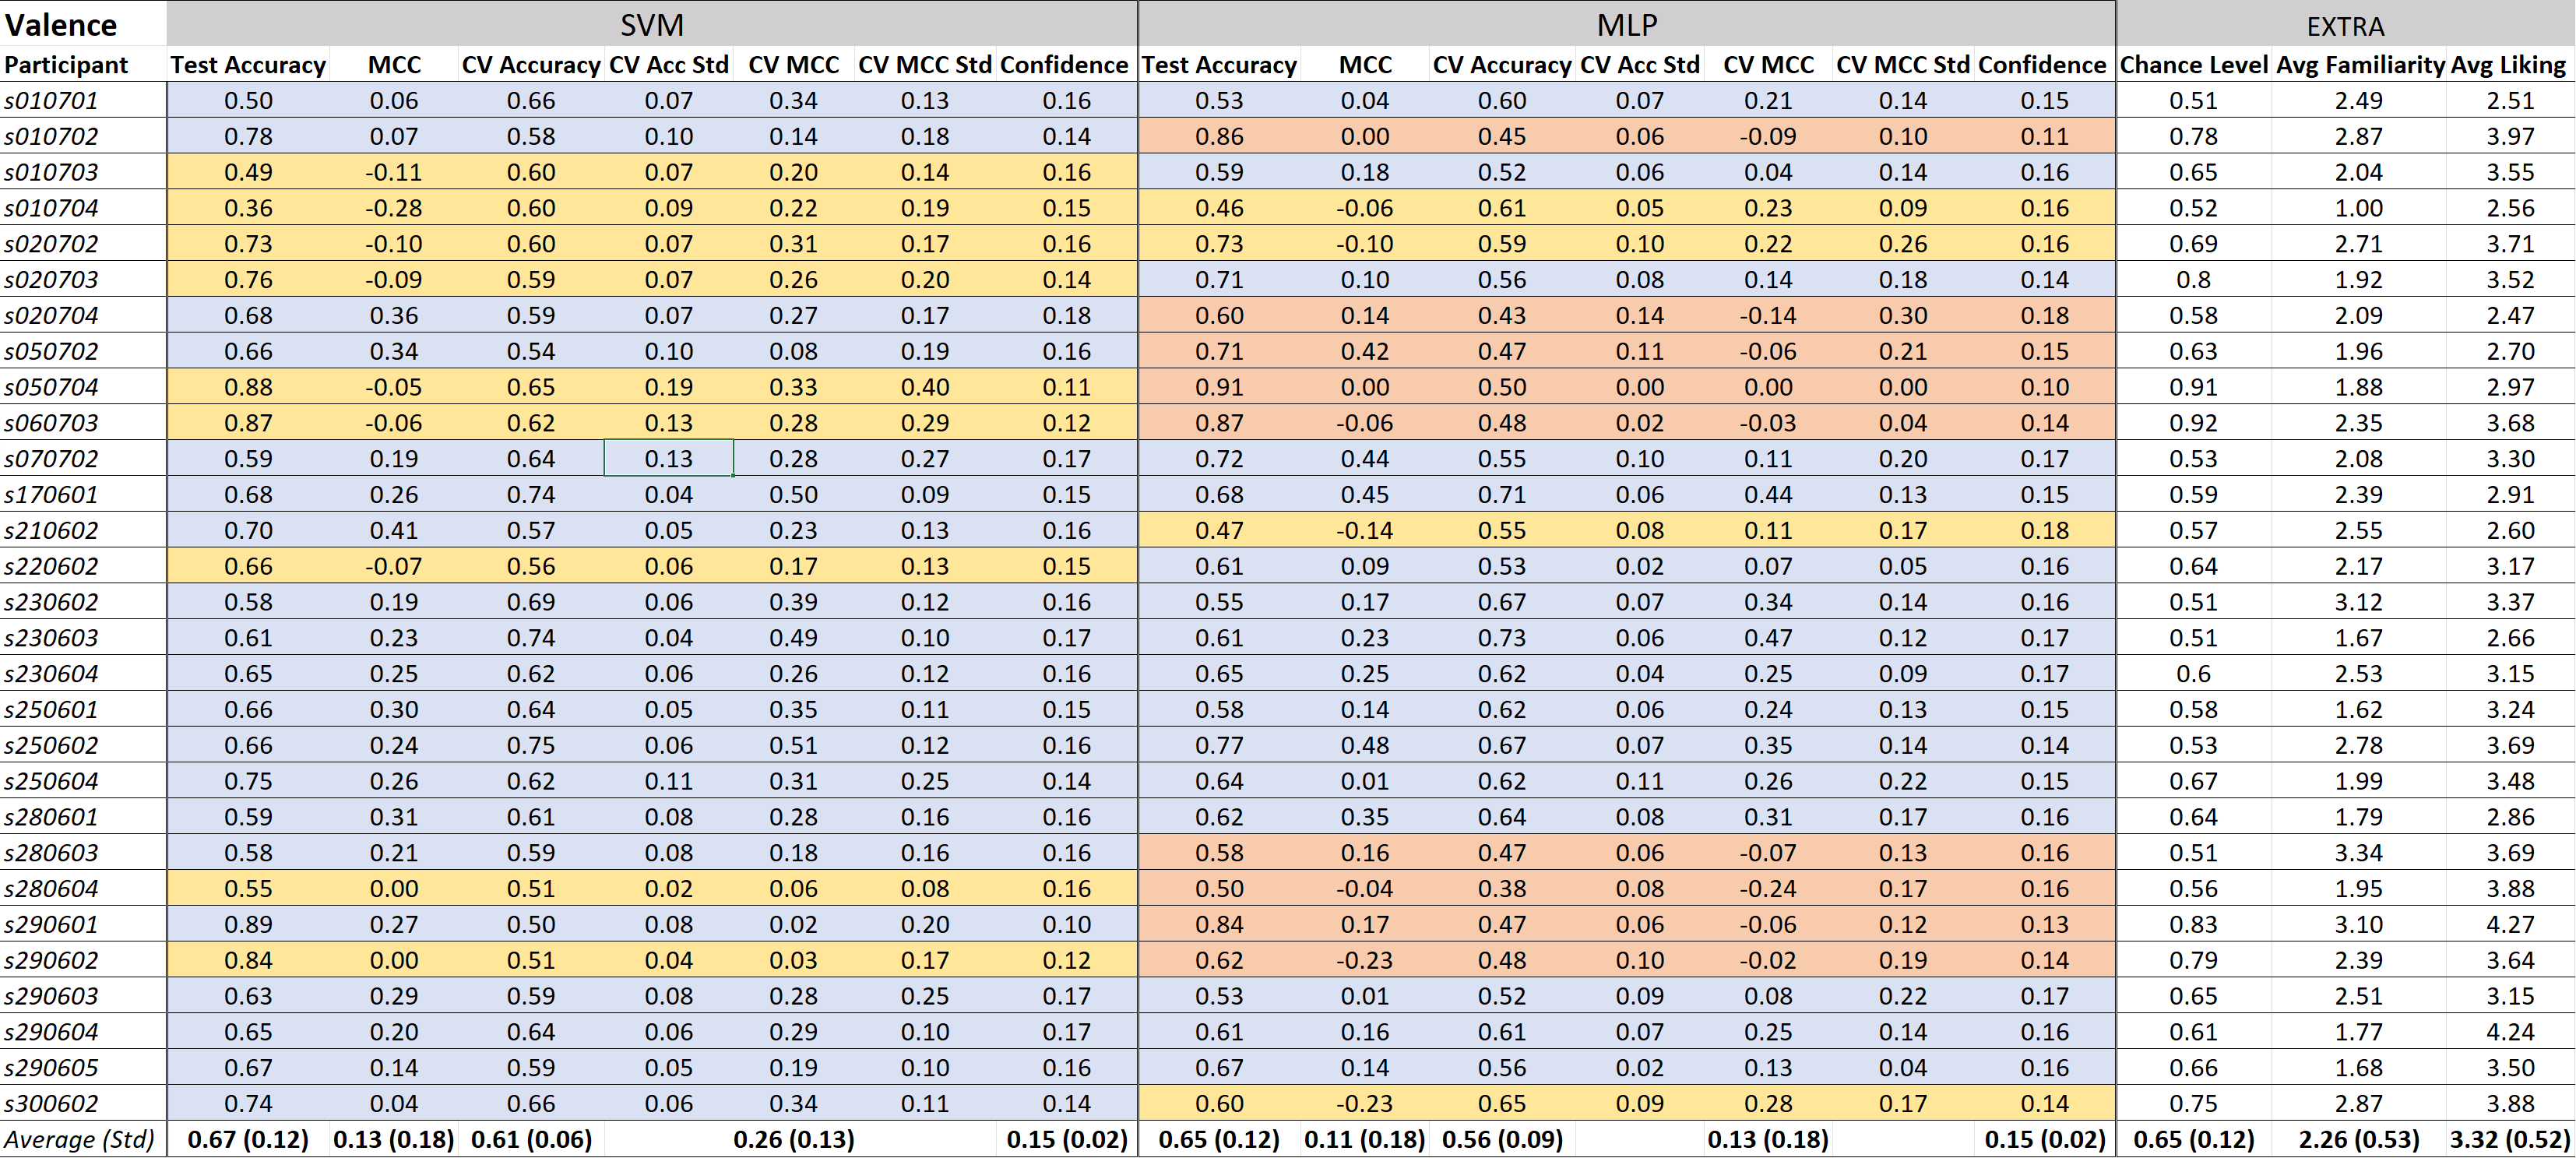
\includegraphics[width=\linewidth]{img/results/valence_results.png}
\end{table}

Overall, the classification performances between \ac{SVM} and \ac{MLP} are not significantly different, except for the Cross-Validated MCC scores that reveal a better learning consistency using \ac{SVM}. Surprisingly, arousal classification resulted in higher absolute accuracy scores and for \ac{SVM} a significantly minor number of not-learning models. This could be explained by the different distribution of labels, which for valence is more unbalanced towards the positive class (see Chapter \ref{sec:unbalanced_labelling}).

\section{Better learning or better accuracy}
\label{sec:better_learning_accuracy}
The same experiment was repeated choosing \emph{accuracy} as scoring parameter for GridSearch when tuning hyper-parameters, with “max accuracy” strategy. The purpose of this experiment was to compare the scoring strategies; however, it is important to underline that the loss function implemented in the scikit-learn library for GridSearch is chosen to optimize accuracy and only then the scoring parameter is used to select the best configuration. The results of subject-dependent arousal classifications are reported in Table 3, and they are not significantly different from the previous experiment. However, the highest consistent accuracy score using \ac{MLP} is 77\% with \ac{MCC} score of 0.53. Furthermore, it is possible to notice an increased number of negative \ac{MCC} and \ac{CV MCC} scores, and for \ac{MLP} the best performing models are not entirely consistent with the previous experiment.

\begin{table}[h!]
  \caption{Arousal classification results using Accuracy as scoring parameter for GridSearch. The 5 best performing models in terms of accuracy and MCC score are highlighted in blue, the models with MCC <= 0 and CV MCC <= 0 are highlighted in orange and yellow, respectively.}
  \label{tbl:arousal_max_acc_results}
  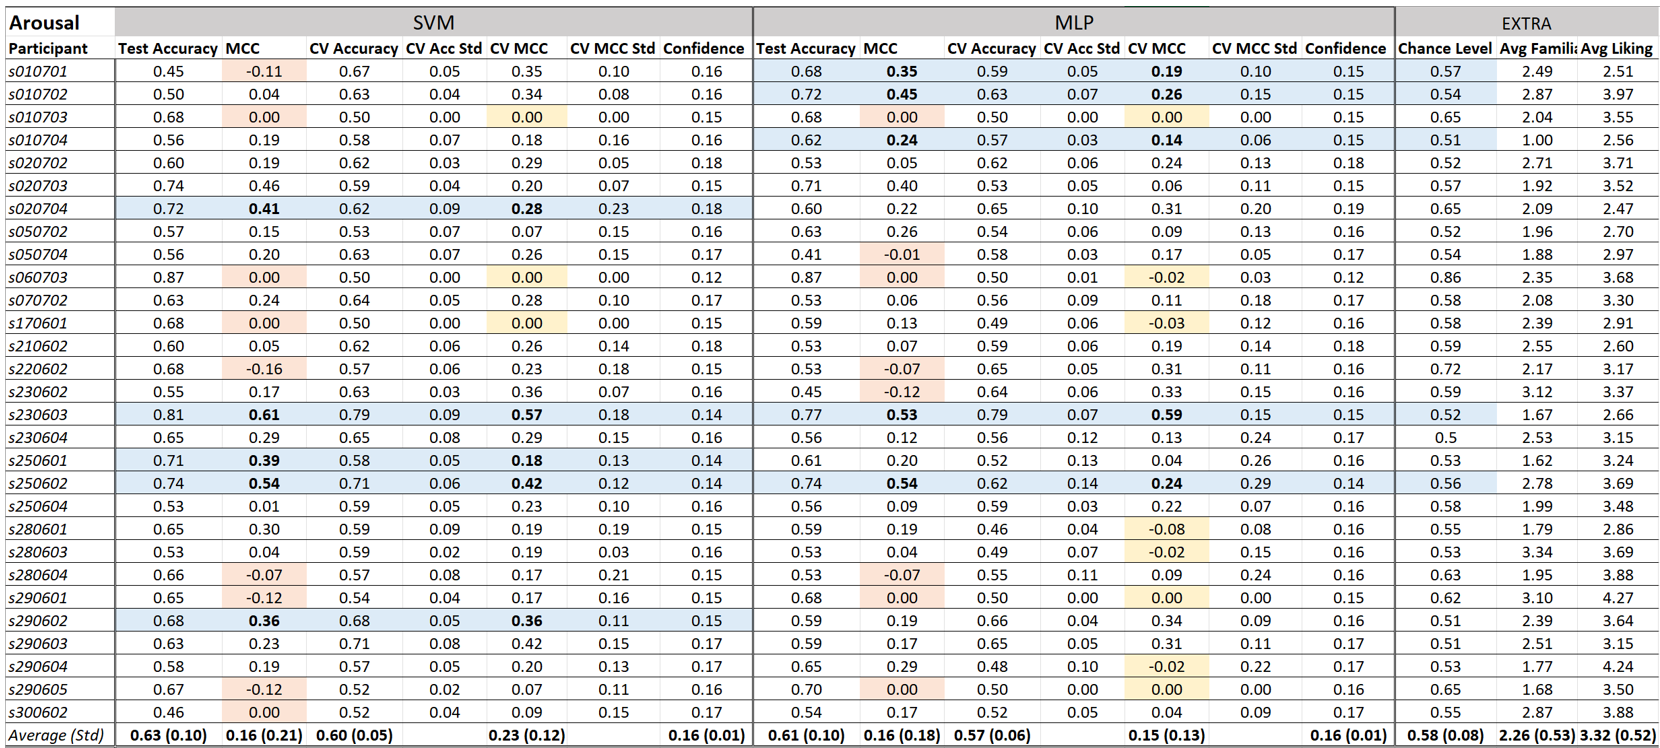
\includegraphics[width=\linewidth]{img/results/arousal_max_acc_results.png}
\end{table}

For valence classification the average test score is slightly higher for both \ac{SVM} and \ac{MLP}, but the highest accuracy score for \ac{MLP} reaches 90\% with \ac{MCC} score of 0.36. For \ac{SVM} the highest accuracy score is 80\% with \ac{MCC} score of 0.11. These highest accuracy scores are not consistent with the previous experiment and the relatively lower associated \ac{MCC} scores can be explained by the different scoring strategy.

\begin{table}[h!]
  \caption{Valence classification results using Accuracy as scoring parameter for GridSearch. The 5 best performing models in terms of accuracy and MCC score are highlighted in blue, the models with MCC <= 0 and CV MCC <= 0 are highlighted in orange and yellow, respectively.}
  \label{tbl:valence_max_acc_results}
  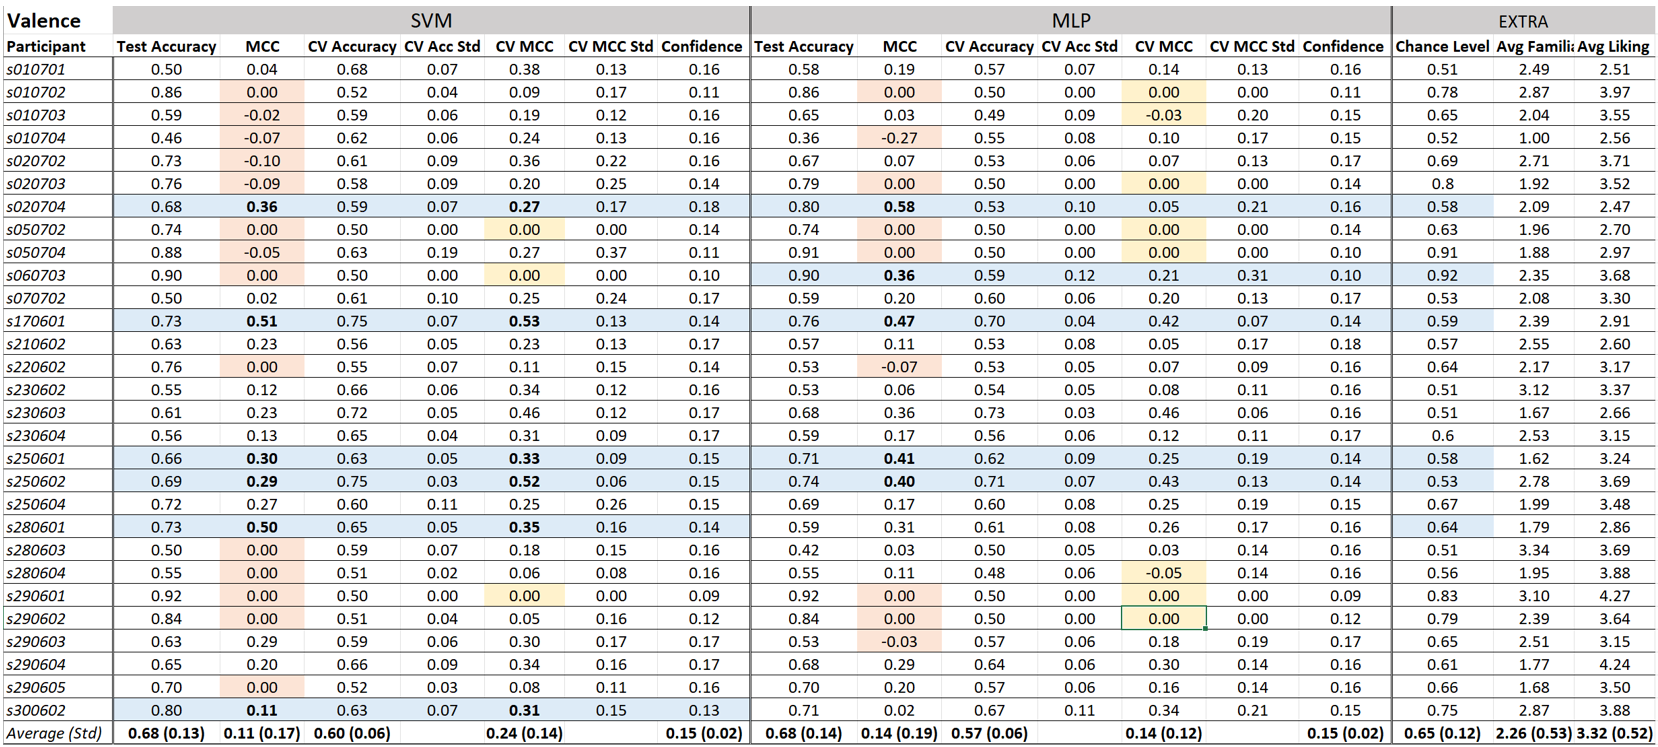
\includegraphics[width=\linewidth]{img/results/valence_max_acc_results.png}
\end{table}

Overall, it is also noticeable that an increased number of models is not learning, either because of over-fitting or under-fitting. This is particularly evident for arousal classification. This can be observed in the plots in Fig. \ref{fig:arousal_strategy_comparison} and Fig. \ref{fig:valence_strategy_comparison}, in which the number of models scoring 0 or less in \ac{MCC} and \ac{CV MCC} scores is compared between both strategies, for arousal and valence respectively.

\begin{figure}[h!]
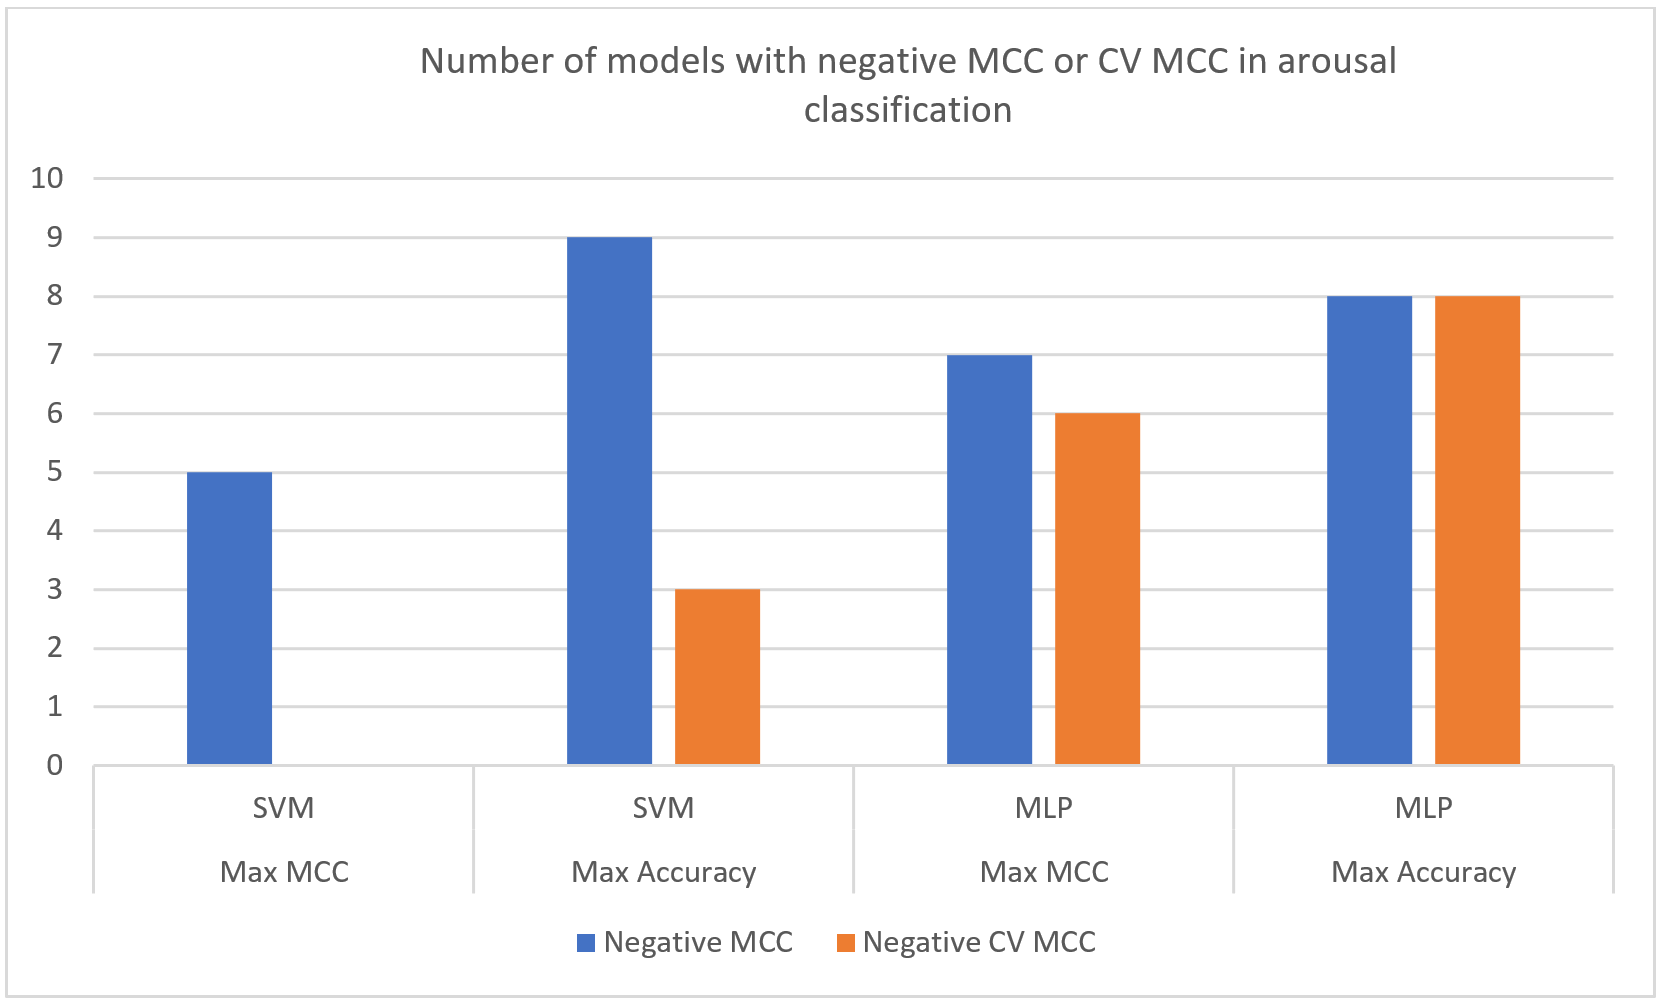
\includegraphics[width=12cm]{img/results/arousal_strategy_comparison.png}
\centering
\caption{Comparison between optimization strategies of negative MCC and CV MCC scores counts for arousal classification.} \label{fig:arousal_strategy_comparison}
\end{figure}

For arousal classification the difference between Max MCC strategy is evident and significant for \ac{SVM} classifiers, and there is increasing trend between Max MCC strategy and Max Accuracy Strategy. In valence classification the difference is less remarkable, but the same increasing trend between the two strategies is present.

\begin{figure}[h!]
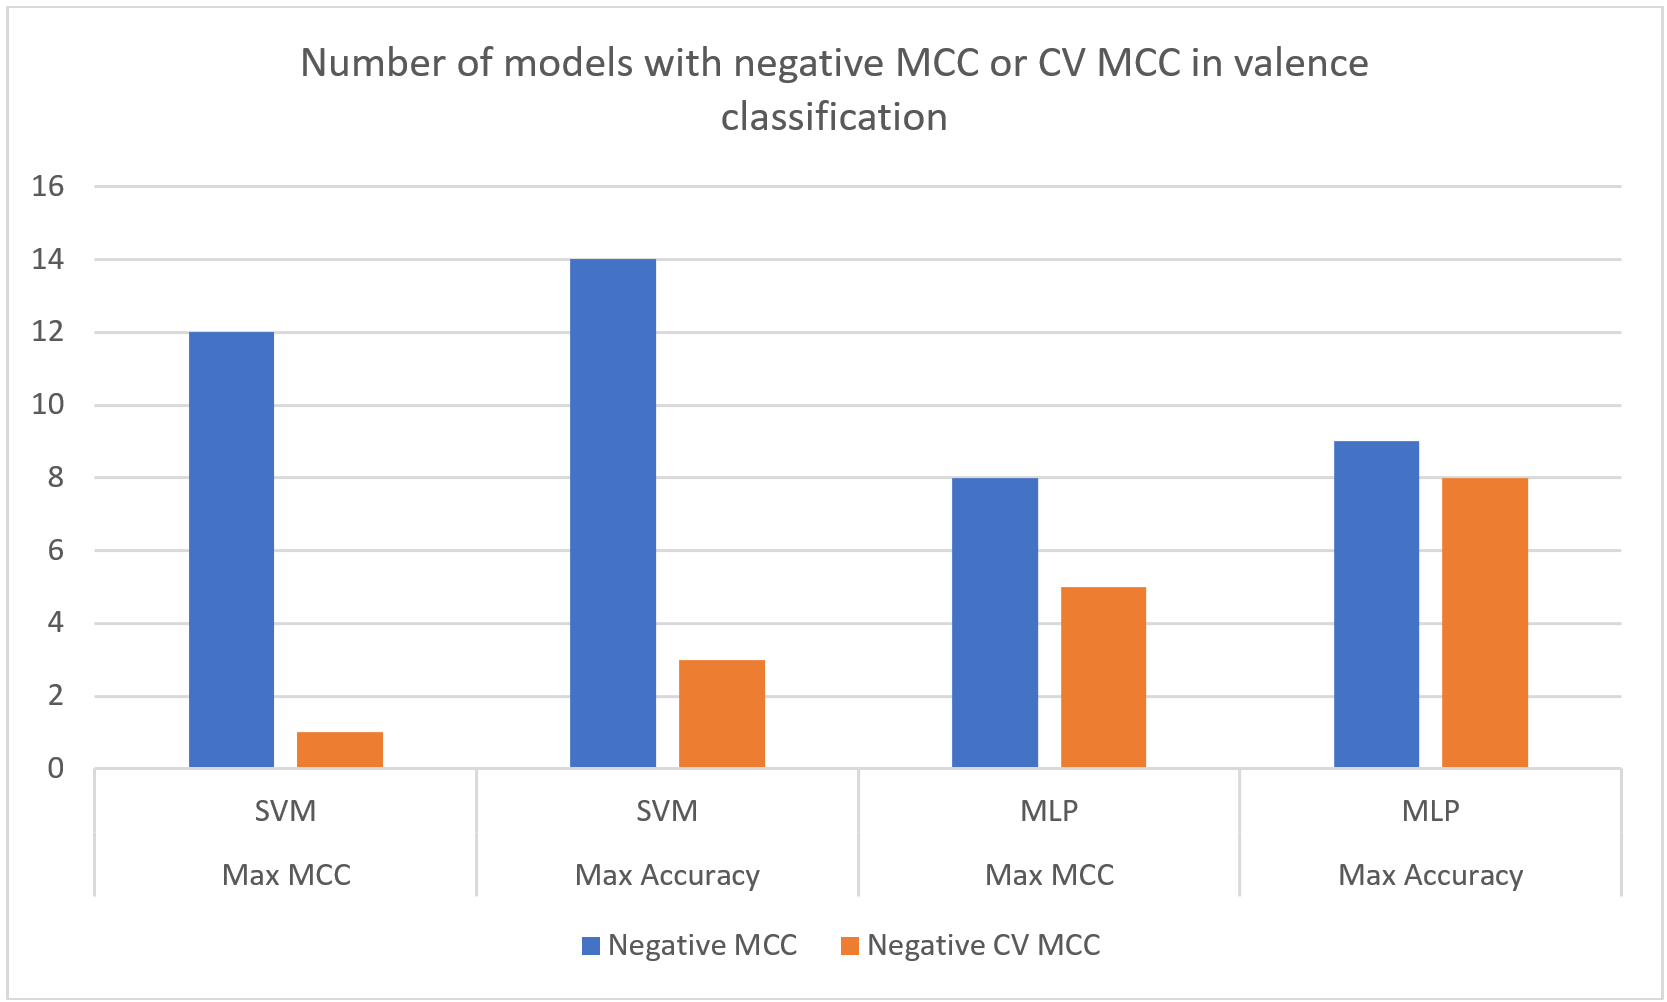
\includegraphics[width=12cm]{img/results/valence_strategy_comparison.png}
\centering
\caption{Comparison between optimization strategies of negative MCC and CV MCC scores counts for arousal classification.} \label{fig:valence_strategy_comparison}
\end{figure}

The current research is more focused on obtaining more interpretable and valid results from the classification of emotional valence and arousal rather than blindly maximizing the accuracy scores of the classifiers. The “Max Accuracy” strategy is less benevolent towards a general approach and generates more over-fitted or under-fitted models than “Max MCC” strategy, therefore results obtained using the latter strategy are considered the final ones and compared with the related work in the following section.

\section{Comparison with related work}
\label{sec:comparison}
Comparing the result of the current research with related work is non-trivial because of the methodological differences in data collection, processing, and evaluation. These differences have been considered to sort the comparisons from most comparable to least comparable. 
\\
The first and most comparable study [31] used self-reported continuous annotation as main labelling method for classification, the data were collected from 9 subjects with a wearable EEG headset equipped with 8 dry electrodes and processed using the automated PREP pipeline in MATLAB. The accuracy scores of SVM classifiers using EEG and LOBO cross-validation are only reported through plots, valence classification scored average accuracy of ~68\% and a standard deviation ~0.10, and arousal classification scored average accuracy ~64\% and a standard deviation ~0.10. The current study reports average test accuracy of 65\% (0.12) and average LOBO cross-validated accuracy on the training set of 61\% (0.07) for valence classification using SVM classifiers. Arousal classification scored an average test accuracy of 63\% (0.09) and average LOBO cross-validated accuracy of 61\% (0.06). They provided a table reporting the MCC scores for each classification modality, the average CV MCC reported for valence is 0.247 (0.17) and the average CV MCC for arousal is 0.177 (0.04). The current study reports average test MCC score of 0.10 (0.15) and average CV MCC score of 0.26 (0.15) for valence, while for arousal the average test MCC score is 0.18 (0.20) and average CV MCC score is 0.24 (0.13). Finally, the individual highest CV MCC score reported is 0.596 (0.3) for valence and 0.23 (0.22) for arousal, while in the current study the highest CV MCC score reported is 0.53 (0.13) for valence and 0.57 (0.18) for arousal, using SVM. These results are aligned with the current study and provide individual insights for each subject that can be easily compared.
\\
The second comparable study [26] is the one that inspired the self-reporting of emotions using continuous annotation. The focus of this study, however, was to compare traditional discrete annotations to continuous annotation and to evaluate two approaches for features extraction. For comparison purposes, the scores reported using PSD features will be considered instead of the scores obtained with FD features. The accuracy scores, and relative standard deviations are mostly reported in plots and partially during the discussion, so an estimate is provided. Using SVM, valence classification score is ~81.2\% (0.08) average CV accuracy and arousal classification score is ~75\% (0.08) average CV accuracy. With MLP, valence classification score is ~80.2\% (0.1) average CV accuracy and arousal classification score is ~75\% (0.1) average CV accuracy. These scores are significantly higher than chance level and clearly outperform the results obtained in the current study, that are not on average significantly higher than chance level. No further insights are provided on individual performances, so they can be considered not relevant. 
\\
The third study [25] aimed at artificially simulating a wearable device by selecting, 2, 4 and then 8 frontal electrodes from the subjects of the DEAP dataset, collected with and EEG system with 32 wet electrodes and discrete self-reported labels. Only the results for the 2 electrodes configuration using SVM for subject-dependent classification are reported and no specific description of the preprocessing pipeline is provided. The average CV accuracy scored for valence classification is ~68.4\% (0.02). The authors also provide better scoring using GBDT classifier for subject-dependent and subject-independent classification and a balancing strategy for the labels is explained, but no specific distribution of positive and negative class is provided, nor individual insights for subject-dependent classification.
\\
The fourth and last comparable study [23] collected self-reported continuous annotations from 26 subjects using a standard EEG system with 32 wet electrodes. The data were preprocessed with visual inspection on EEG lab and then features were extracted from 12 pairs of symmetrical electrodes. The authors provide 3 classifications schemes, but only the “one-against-one scheme is comparable in terms of binary classification of valence and arousal and therefore reported. The reported CV accuracy score for valence classification is 94.86\% (0.176) and for arousal classification is 94.43\% (0.212). The authors did not report the distribution of the classes.
